\documentclass[12pt,letterpaper]{article}

% ---------- Encoding, fonts, layout ----------
\usepackage[T1]{fontenc}
\usepackage[utf8]{inputenc}

  \usepackage{newtxtext, newtxmath}

\usepackage{geometry}
\geometry{margin=1in}

\usepackage{microtype}
\usepackage{setspace}
\setstretch{1.15}
\setlength{\parskip}{6pt plus 2pt minus 1pt}
\setlength{\parindent}{0pt}
\setlength{\emergencystretch}{3em}

\usepackage{tabularx}
\newcolumntype{Y}{>{\raggedright\arraybackslash}X}

% ---------- Graphics & tables ----------
\usepackage{graphicx}
\usepackage{booktabs}
\usepackage{longtable}
\usepackage{array}
\usepackage{float} % <-- enables [H] float placement
\IfFileExists{footnote.sty}{\usepackage{footnote}\makesavenoteenv{longtable}}{}

% 
% ---------- Links ----------
\usepackage{xcolor}
\definecolor{linkblue}{rgb}{0.0,0.2,0.6}
\usepackage{hyperref}
\hypersetup{
  colorlinks=true,
  linkcolor=linkblue,
  citecolor=linkblue,
  urlcolor=linkblue,
  breaklinks=true,
  pdftitle={},
  pdfauthor={}
}
\urlstyle{same}

% ---------- Header / footer ----------
\usepackage{fancyhdr}
\pagestyle{fancy}
\fancyhf{}

% Use shorttitle from YAML; fall back to full title if not provided
\newcommand{\ShortTitleText}{NPT Proposed Weir Management}

% Default (all pages except the first): short title on the left, page number right
\lhead{\textsf{\ShortTitleText}}
\rhead{\textsf{\thepage}}
\setlength{\headheight}{15pt}
\renewcommand{\headrulewidth}{0.4pt}  % horizontal rule ON for subsequent pages

% First-page style: NO header rule, NO page number
\fancypagestyle{firstpage}{
  \fancyhf{}                 % clear header/footer
  \renewcommand{\headrulewidth}{0pt} % remove the line on first page
}

% ---------- Section titles (valid separation lengths) ----------
% ---------- Section titles (unnumbered) ----------
\setcounter{secnumdepth}{0}  % do not number sections at all

\usepackage[compact,sf,bf]{titlesec}
\titleformat{\section}[block]{\Large\bfseries\sffamily}{}{0.6em}{}        % no \thesection
\titleformat{\subsection}[block]{\normalsize\bfseries\sffamily}{}{0.5em}{} % no \thesubsection
\titleformat{\subsubsection}[block]{\normalsize\bfseries\sffamily}{}{0.5em}{}

\titlespacing{\section}{0pt}{*2}{*0.6}
\titlespacing{\subsection}{0pt}{*1.2}{*0.4}
\titlespacing{\subsubsection}{0pt}{*1.0}{*0.3}


% ---------- Captions ----------
\usepackage{caption}
\DeclareCaptionStyle{italic}[justification=raggedright,singlelinecheck=false]{labelfont={bf},textfont={it},labelsep=colon}
\captionsetup[figure]{style=italic,format=hang}
\captionsetup[table]{style=italic,format=hang}

% ---------- BibLaTeX (enabled only if bibliography is provided) ----------
\usepackage[style=authoryear-comp,backend=biber,natbib=true,maxnames=3]{biblatex}
\addbibresource{../anchor_memo.bib}

% ---------- BibLaTeX (enabled only if bibliography is provided) ----------
% Configure BibLaTeX for American Fisheries Society (AFS) style
% \PassOptionsToPackage{
%   backend=biber,     % Core processing engine
%   style=authoryear,  % Author-Year format
%   maxcitenames=2,    % Use 'et al.' for more than 2 authors in text
%   maxbibnames=99,    % List all authors in the bibliography
%   uniquename=false,  % Turn off initials for conflicting last names
%   uniquelist=false
% }{biblatex}
% 
% % AFS Specific Tweaks:
% \AtBeginDocument{
%   % Remove the comma between Author and Year in text citations: e.g., (Kinzer 2026)
%   \DeclareDelimFormat{nameyeardelim}{\addspace} 
%   
%   % Separate multiple entries with semicolons: e.g., (Kinzer 2026; Briggs 2025)
%   \DeclareDelimFormat{multicitedelim}{\addsemicolon\space}
% }


% ---------- Optional watermark ----------
\usepackage{draftwatermark}
\SetWatermarkText{DRAFT}
\SetWatermarkScale{0.9}
\SetWatermarkColor[gray]{0.9}

% ---------- tcolorbox (memo header + callouts) ----------
\usepackage[most]{tcolorbox}
\tcbset{boxrule=0.5pt,arc=2mm,left=6pt,right=6pt,top=6pt,bottom=6pt}

% Executive Summary / Recommendations environments (optional)
\newenvironment{execsum}{%
  \begin{tcolorbox}[colback=blue!3,colframe=blue!50!black,title=\textbf{Executive Summary}]
}{\end{tcolorbox}}

\newenvironment{recs}{%
  \begin{tcolorbox}[colback=green!3,colframe=green!40!black,title=\textbf{Recommendations}]
}{\end{tcolorbox}}

% ---------- Branding (logos), only if branding: yes ----------
\usepackage[absolute,overlay]{textpos}
\setlength{\TPHorizModule}{1cm}
\setlength{\TPVertModule}{1cm}

% ---------- Memo header box ----------
\newcommand{\MemoHeader}{%
      \vspace*{2cm}% push content down if branding block is present
    \begin{tcolorbox}[colback=gray!5,colframe=gray!45,coltitle=black, center title, title=\textbf{Technical Memorandum}]
    \begin{tabularx}{\textwidth}{@{}p{2.2cm} Y@{}}
      \textbf{To} &
        \begin{minipage}[t]{\linewidth}\raggedright
          \setlength{\parindent}{0pt}%
          Jason Vogel, DFRM Research Division Director\\ William Young, DFRM Hatchery Evaluations Coordinator\\ Becky Johnson, DFRM Production Division Director
        \end{minipage}
      \\
      \textbf{From} &
        \begin{minipage}[t]{\linewidth}\raggedright
          \setlength{\parindent}{0pt}%
          Ryan N. Kinzer, DFRM Fisheries Data Analysis Coordinator
        \end{minipage}
      \\
            \textbf{CC} &
        \begin{minipage}[t]{\linewidth}\raggedright
          \setlength{\parindent}{0pt}%
          Brian Simmons, DFRM Research RM\&E Lead
        \end{minipage}
      \\
            \textbf{Date}    & 28 August, 2026 \\
      \textbf{Subject} & NPT's Proposed North East Oregon Weir Management Framework Using HSRG Recommendations \\
      
      
    \end{tabularx}
  \end{tcolorbox}
}


% ---------- Title metadata ----------
  \title{}

  \author{%
          \textbf{}\\
          }

\date{28 August, 2026}

% --- Pandoc tight list shim (prevents \tightlist error) ---
\providecommand{\tightlist}{%
  \setlength{\itemsep}{0pt}\setlength{\parskip}{0pt}}

% -------------------- BODY --------------------
\begin{document}

% Branding logos (optional)
  \begin{textblock}{3}(1,1.1)
\includegraphics[height=2.0cm]{../../templates/NPT.png}\end{textblock}
   \begin{textblock}{14}(3.75,0.5)
      \begin{center}
        {\LARGE Nez Perce Tribe}\\[0.1em]
        {\bfseries\Large Department of Fisheries Resources Management}\\[0.1em]
        {\bfseries\footnotesize Administration \textbullet Enforcement \textbullet Habitat/Watershed \textbullet Harvest \textbullet Production \textbullet Research}\\[0.1em]
        {\bfseries\normalsize Research Division}\\[0.1em]
        {\footnotesize P.O. Box 365 \textbullet Lapwai, Idaho 83540}\\[0.1em]
        {\footnotesize Phone: (208) 843-7145 \textbullet Fax: (208) 843-7310}\\[0.1em]        
      \end{center}
    \end{textblock}
  \begin{textblock}{3}(19,1.1)
\includegraphics[height=2.0cm]{../../templates/DFRM.png}\end{textblock}

% (Small title for PDF metadata clarity)
{\large\bfseries\sffamily }\par\vspace{0.4em}

% Make the FIRST page clean: no line, no page number
\thispagestyle{firstpage}

% Memo header
\MemoHeader

% Optional Executive Summary / Recommendations if provided via variables


% Content injection hooks

\section{Background}\label{background}

The Lostine River spring Chinook (Oncorhynchus tshawytscha) hatchery program is an integrated supplementation program intended to rebuild and maintain the naturally spawning population while providing harvest opportunities and meeting Tribal and mitigation obligations \autocite{npt_hatchery_2011}. Achieving these objectives requires balancing the demographic benefits of supplementation with potential genetic risks associated with hatchery production and hatchery-origin fish spawning naturally.

The existing sliding-scale framework addresses this balance primarily through natural-origin abundance. At low abundance, demographic risk is emphasized and relatively greater hatchery contribution to natural spawning is allowed. As natural-origin abundance increases, management progressively shifts toward increasing natural-origin broodstock and reducing hatchery-origin spawning. This general approach recognizes an important biological principle: the appropriate balance between demographic support and management of hatchery influence should change as a population progresses toward recovery.

Since the sliding scale was developed, more explicit guidance has become available for managing hatchery programs. The Hatchery Scientific Review Group (HSRG) developed recommendations that consider both a population's historical importance and contribution to the Evolutionarily Significant Unit (ESU) or Distinct Population Segment (DPS), and its current abundance relative to population goals \autocite{hsrg_implementation_2017}. The intersection of these components is used to establish recommended management targets for the proportion of natural-origin fish in the hatchery broodstock (pNOB), the proportion of hatchery-origin fish on the spawning grounds (pHOS), and proportionate natural influence (PNI). Collectively, these metrics describe the potential relative influence of natural and hatchery environments on an integrated population and provide a framework for managing hatchery genetic influence as population status improves.

The underlying HSRG concept is consistent with the biological rationale of the existing sliding scale but provides an opportunity to more explicitly connect management actions with population status and recovery objectives. Rather than relying solely on fixed abundance thresholds developed when the HGMP was established and prior to the adoption of regional and co-manager-approved abundance goals \autocite{cbp_vision_2020}; management objectives can now be defined based on the population's current status relative to those goals. Under this approach, expectations for broodstock composition and hatchery influence become progressively more restrictive as natural abundance increases and the population advances toward recovery.

Application of the HSRG framework to an integrated supplementation program also raises questions about how hatchery influence should be measured. Conventional PNI treats all hatchery-origin adults spawning naturally as representing full segregated hatchery influence, regardless of the ancestry of those fish. In a highly integrated program, however, hatchery-origin adults may be produced from broodstock composed partly or predominantly of natural-origin parents. Treating those adults equivalently to hatchery-origin fish produced entirely from hatchery-origin parents may overstate the potential negative influence of the hatchery environment and does not explicitly account for differences among generations in broodstock integration.

More than a decade of Lostine River monitoring provides an opportunity to incorporate these concepts into a revised management framework. Long-term information on adult abundance, broodstock composition, hatchery-origin spawning, and population performance can now be considered alongside established recovery goals and contemporary guidance for integrated hatchery programs.

The purpose of this memorandum is therefore to propose an updated framework for Lostine River weir management that more explicitly links management actions to population status, recovery objectives, and the degree of hatchery integration. Two related approaches are proposed:

\begin{enumerate}
\def\labelenumi{\arabic{enumi}.}
\tightlist
\item
  Recovery-based weir management. Align and expand upon HSRG recommendations by establishing management expectations for pNOB, pHOS, and PNI that change according to population recovery phase.
\item
  Parental-adjusted natural influence. Evaluate an alternative calculation of PNI in which the contribution of hatchery-origin natural spawners is weighted according to the natural-origin contribution of their parents.
\end{enumerate}

Together, these approaches provide a framework for transitioning management priorities as the population progresses from demographic preservation and recolonization toward local adaptation and full restoration, while more explicitly accounting for the biological characteristics of an integrated supplementation program.

\section{Objective 1: Expanding the HSRG Recovery Framework}\label{objective-1-expanding-the-hsrg-recovery-framework}

The HSRG developed a biological framework for integrating hatchery, harvest, habitat, and hydrosystem management within salmon recovery planning \autocite{hsrg_implementation_2017}. Rather than viewing hatchery reform as a fixed management strategy, the HSRG recommends that hatchery objectives evolve as populations recover. Management actions should therefore reflect both the biological significance of a population to recovery of the ESU/DPS and its current stage of biological recovery \autocite{hsrg_implementation_2017}.

\subsection{Population Significance}\label{population-significance}

The HSRG recommends classifying populations according to their biological significance to ESU recovery. Population significance determines the long-term conservation objectives expected for each population and reflects its contribution toward overall ESU viability.

\begin{itemize}
\tightlist
\item
  \textbf{Primary populations} must ultimately achieve high viability and represent populations of greatest importance to ESU recovery.
\item
  \textbf{Contributing populations} must achieve at least medium viability and contribute to the abundance, diversity, and resilience of the ESU.
\item
  \textbf{Stabilizing populations} are expected to maintain their current viability while continuing to contribute to the genetic and spatial diversity of the ESU.
\end{itemize}

\subsection{Biological Recovery Phases}\label{biological-recovery-phases}

Independent of population significance, the HSRG recognizes four biological recovery phases that describe the progression of a population toward recovery.

\begin{itemize}
\tightlist
\item
  \textbf{Preservation} -- prevent extinction while maintaining genetic diversity.
\item
  \textbf{Recolonization} -- rebuild populations throughout suitable habitat as habitat conditions improve.
\item
  \textbf{Local Adaptation} -- increase natural productivity, reproductive success, and life-history diversity while progressively reducing hatchery influence.
\item
  \textbf{Full Restoration} -- maintain viable, naturally self-sustaining populations that satisfy all Viable Salmonid Population (VSP) parameters through adaptive management.
\end{itemize}

Rather than prescribing fixed criteria, the HSRG recommends developing triggers that transition between recovery phases based on biological indicators that may include abundance, productivity, habitat conditions, spatial structure, and diversity. These triggers should be developed specifically for each population and refined as additional biological information becomes available.

\subsection{Proposed Recovery Phase Thresholds}\label{proposed-recovery-phase-thresholds}

Although the HSRG framework provides a biologically sound conceptual approach, it does not establish standardized quantitative criteria for assigning populations to recovery phases. We propose adopting abundance-based thresholds, based on Columbia Basin Partnership Goals \autocite{cbp_vision_2020}, to provide a transparent and repeatable method for classifying populations while remaining consistent with the HSRG emphasis on biological triggers \autocite{hsrg_developing_2020}.

Specifically, we propose the following operational thresholds:

\begin{itemize}
\tightlist
\item
  \textbf{Preservation:} natural-origin abundance less than the ICTRT Minimum Abundance Threshold (MAT) and the Columbia Basin Partnership (CBP) low abundance goal.
\item
  \textbf{Recolonization:} abundance between the CBP low and medium abundance goals.
\item
  \textbf{Local Adaptation:} abundance between the CBP medium and high abundance goals.
\item
  \textbf{Full Restoration:} abundance exceeding CBP high abundance goals.
\end{itemize}

\subsection{Existing HSRG Broodstock Guidance}\label{existing-hsrg-broodstock-guidance}

For integrated hatchery programs, the HSRG recommends that management priorities differ among recovery phases (Figure \ref{fig:hsrg-management-matrix}).

During the \textbf{Preservation} and \textbf{Recolonization} phases, no formal pHOS or PNI objectives are recommended. Instead, hatchery managers are encouraged to maximize the use of natural-origin broodstock whenever feasible while allowing all remaining hatchery-origin fish to contribute to natural spawning.

As populations transition into the \textbf{Local Adaptation} and \textbf{Full Restoration} phases, management emphasis shifts toward reducing hatchery influence and promoting local adaptation. At this stage, broodstock and natural spawning are managed to satisfy pHOS and PNI objectives that vary according to population significance.

Numeric guidelines for pHOS and PNI managment targets were developed to balance genetic and demographic concerns \autocite{hsrg_implementation_2017}. Generally, management targets shift from allowing more HOR fish to spawn naturally and into the brood stock, to a more stringent approach seeking to reduce HOR influence on the population (Figure \ref{fig:hsrg-management-matrix}).

\begin{figure}[H]

{\centering 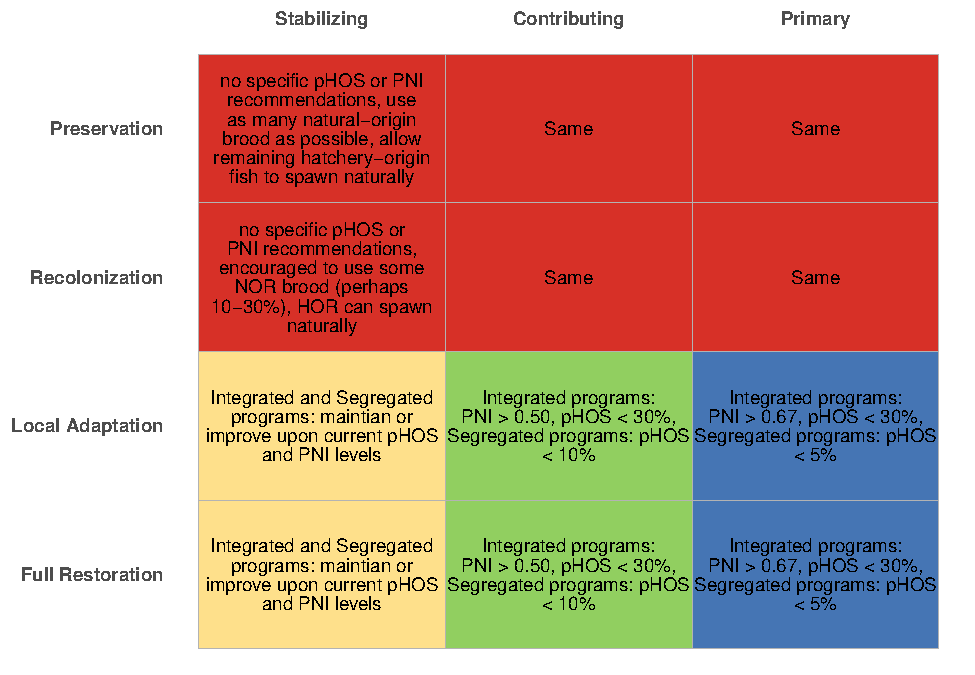
\includegraphics[width=1\linewidth]{NEOR_proposed_weir_mgt_files/figure-latex/hsrg-management-matrix-1} 

}

\caption{HSRG recommended hatchery weir management framework based on biological recovery phase and population significance.}\label{fig:hsrg-management-matrix}
\end{figure}

\subsection{Proposed Two-Dimensional Decision Framework}\label{proposed-two-dimensional-decision-framework}

The HSRG framework considers population significance and biological recovery as complementary concepts. However, current broodstock recommendations primarily depend on population significance once populations reach the Local Adaptation phase. We propose integrating both designations into a single management framework.

Under the proposed approach, broodstock collection and natural spawning objectives would be determined jointly by:

\begin{enumerate}
\def\labelenumi{\arabic{enumi}.}
\tightlist
\item
  \textbf{Population significance}, representing the long-term biological importance of the population to ESU recovery; and
\item
  \textbf{Biological recovery phase}, representing the current status of the population relative to recovery goals.
\end{enumerate}

This two-dimensional framework recognizes that management priorities should evolve continuously throughout recovery rather than changing only after populations exceed a single abundance threshold. Early recovery phases should prioritize increasing abundance and reducing extinction risk, whereas later phases should progressively emphasize local adaptation, natural productivity, and the long-term reduction of hatchery influence.

The proposed framework provides managers with greater flexibility to balance harvest, broodstock collection, natural production, and genetic considerations while maintaining consistency with the overarching objectives of the HSRG recovery strategy.

\subsection{Example Management Matrix}\label{example-management-matrix}

Figure \ref{fig:proposed-management-matrix} provides an example management matrix that uses CBP abundance goals as thresholds between biological recovery phases. The specific management targets (e.g., pHOS, pNOB, and PNI) associated with each cell of the matrix should be developed collaboratively using population-specific biological information and adaptive management. Rather than prescribing precise management targets at specific annual abundances, as occurs under the current sliding scale, the matrix provides a structured framework for integrating population recovery status and population significance to guide hatchery management within biologically acceptable and operationally achievable ranges.

Overall, this approach extends the HSRG framework by explicitly recognizing that broodstock management should evolve as populations recover. Defining biological recovery phases within the context of regionally accepted recovery goals and integrating those phases with population significance provides managers with a more transparent and biologically defensible framework for balancing conservation, harvest, and supplementation objectives while remaining consistent with long-term recovery goals.

\begin{figure}[H]

{\centering 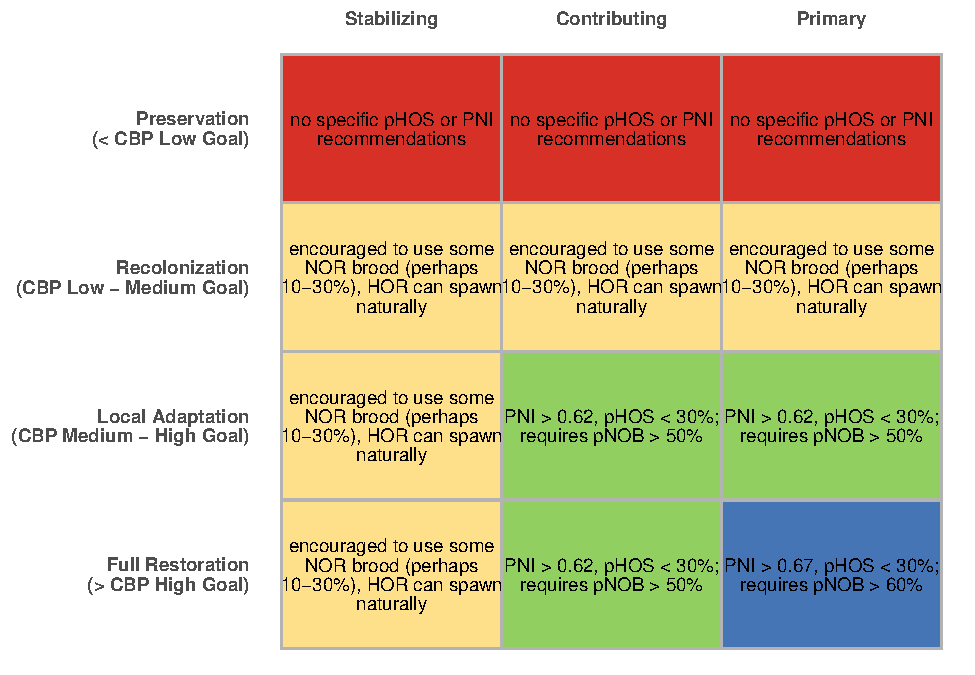
\includegraphics[width=1\linewidth]{NEOR_proposed_weir_mgt_files/figure-latex/proposed-management-matrix-1} 

}

\caption{Proposed Example two-dimensional hatchery-management framework based on biological recovery phase and population significance.}\label{fig:proposed-management-matrix}
\end{figure}

\subsection{Application to North East Oregon Populations}\label{application-to-north-east-oregon-populations}

To provide management stability and avoid changes in weir operations resulting from annual fluctuations in abundance or uncertainty in in-season forecasts, population recovery phase should be based on a multi-year measure of abundance rather than a single-year estimate. This would allow weir management to be based on a more stable assessment of population status and reduce the likelihood that short-term fluctuations in adult returns would result in frequent movement among recovery phases.

One potential approach would be to use the 10-year geometric mean abundance reported in the most recent Endangered Species Act (ESA) 5-year status review to determine recovery phase. In addition to smoothing annual variation in abundance, this approach would directly link hatchery management decisions with the population assessments used by NOAA Fisheries to evaluate ESA status and recovery.

The Imnaha River and Lostine River populations are designated as primary populations with proposed recovery objectives of highly viable or low risk of extinction {[}\textcite{noaa_esa_2017}; Table 4-1{]}. In the most recent ESA 5-year status review, the 10-year geometric mean abundance for both populations was below the CBP Low Goal \autocite{ford_biological_2022}. Under the proposed framework, both populations would therefore currently be classified in the Recolonization recovery phase. Management during this phase would emphasize rebuilding natural-origin abundance, with no specific limits on pHOS or PNI (Figure \ref{fig:proposed-management-matrix}).

\section{Objective 2: Parental-Adjusted Proportionate Natural Influence}\label{objective-2-parental-adjusted-proportionate-natural-influence}

The proportionate natural influence (PNI) is widely used to evaluate integrated hatchery programs because it provides a simple index of the relative influence of natural and hatchery selection on a population. Operationally, PNI combines the proportion of natural-origin broodstock (pNOB) with the proportion of hatchery-origin fish spawning naturally (pHOS) to approximate the relative strength of natural and hatchery influence (Figure \ref{plot-pni-surface}). PNI is therefore a management proxy rather than a direct measure of the biological effects of hatchery-origin fish on natural populations. Direct evaluation of effects on population productivity and fitness is more appropriately accomplished through parentage analyses, relative reproductive success (RRS) studies, and other demographic and genetic investigations that quantify the reproductive performance and long-term contribution of hatchery- and natural-origin fish.

The traditional PNI is calculated as

\[
PNI_t=
\frac{pNOB_t}
{pNOB_t+pHOS_t},
\]

where

\[
pNOB_t=
\frac{Natural\text{-}origin\ broodstock_t}
{Total\ broodstock_t},
\]

and

\[
pHOS_t=
\frac{Hatchery\text{-}origin\ spawners_t}
{Natural\text{-}origin\ spawners_t+Hatchery\text{-}origin\ spawners_t}.
\]

This formulation provides a practical accounting metric for comparing the relative contributions of natural-origin broodstock and hatchery-origin natural spawners. However, it implicitly treats all hatchery-origin fish spawning naturally as equivalent sources of hatchery influence, regardless of the brood year from which they originated or the composition of the broodstock that produced them. This simplification may become increasingly important in mature integrated supplementation programs that have intentionally incorporated natural-origin adults into hatchery broodstock over multiple generations. Under these programs, returning hatchery-origin adults may differ substantially in their parental history and, consequently, in the relative influence of natural and hatchery selection experienced by their parental generation.

\begin{figure}[H]

{\centering 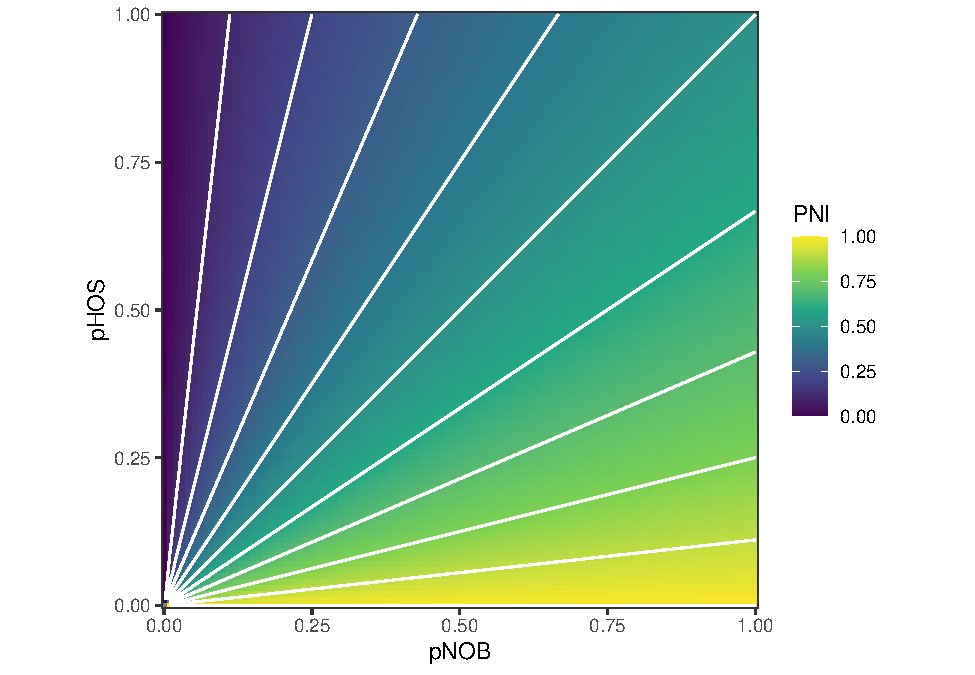
\includegraphics[width=1\linewidth]{NEOR_proposed_weir_mgt_files/figure-latex/plot-pni-surface-1} 

}

\caption{Proportion of natural influence (PNI) response to possible values of proportion of natural-origin brood (pNOB) and proportion of hatchery-origin spawners.}\label{fig:plot-pni-surface}
\end{figure}

A simple example illustrates this limitation. Suppose 100 age-4 adults return in year \(t+4\), consisting of 25 natural-origin and 75 hatchery-origin fish. If 10 natural-origin and 25 hatchery-origin adults are collected for broodstock, the resulting values are \(pNOB = 0.29\), \(pHOS = 0.77\), and \(PNI = 0.27\). Under the traditional formulation, each of the hatchery-origin fish spawning naturally contributes equally to pHOS and, consequently, to the estimated hatchery influence on the population.

However, suppose the hatchery-origin adults returning in year \(t+4\) were produced from a brood year in which hatchery broodstock consisted entirely of natural-origin adults (\(pNOB_t = 1.0\)) and no hatchery-origin adults spawned naturally (\(pHOS_t = 0.0\)). Under the conventional PNI framework, that parental generation would have had \(PNI_t = 1.0\). Nevertheless, when its hatchery-origin offspring return four years later, conventional PNI treats them identically to hatchery-origin adults produced from a parental generation with substantially lower pNOB and PNI. Thus, information about the degree of integration achieved in the parental generation is lost when PNI is calculated for the returning generation.

One potential extension is to replace the conventional pHOS term with a parental-influence-adjusted pHOS, in which returning hatchery-origin adults are weighted according to the broodstock composition and natural spawning conditions of the brood year that produced them. Rather than treating all hatchery-origin adults as equivalent sources of hatchery influence, each returning cohort would contribute to the adjusted pHOS term according to the relative natural and hatchery influence represented by its parental generation. This approach would retain the basic structure and management utility of PNI while incorporating information about the multigenerational integration of natural- and hatchery-origin fish.

\subsection{Conceptual Framework}\label{conceptual-framework}

Under the proposed framework, hatchery-origin fish are no longer treated as having identical hatchery influence. Instead, the influence assigned to each returning cohort is determined by the parental conditions that produced that cohort. Consequently, two hatchery-origin fish returning in the same year may contribute differently to hatchery influence if they originated from different brood years or experienced different parental histories.

This approach recognizes that integrated supplementation programs are inherently multigenerational. Management decisions made during one brood year influence the composition and characteristics of hatchery-origin adults returning several years later. Consequently, the hatchery influence associated with a returning adult should be viewed as a cumulative property of its parental history rather than solely a function of its hatchery origin. Hatchery-origin fish produced from broodstock composed primarily of natural-origin adults should therefore represent a different level of hatchery influence than hatchery-origin fish produced from broodstock with relatively low natural-origin representation. Rather than assuming that hatchery influence is reset each generation, the proposed framework explicitly carries parental influence forward through successive cohorts.

To account for these differences, each brood year is assigned a parental influence weight, (w\_b), where (b) denotes the brood year. The weight represents the relative hatchery influence associated with the parental generation and is bounded between 0 and 1. Values approaching 0 represent brood years produced under predominantly natural influence, whereas values approaching 1 represent brood years produced under relatively greater hatchery influence.

The weighting function is intentionally left general. It may ultimately be derived from one or more measures describing the parental generation, including broodstock composition, natural spawning composition, parentage analyses, relative reproductive success, pedigree reconstruction, or combinations thereof. In general,

\[
w_b=f(x_b),
\]

where (\(x_b\)) represents the biological information available for brood year (b). Possible formulations include

\[
w_b=f(pNOB_b,pHOS_b),
\]

\[
w_b=f(PNI_b),
\]

or, when sufficient pedigree information becomes available,

\[
w_b=f(RRS_b),
\]

where (RRS\_b) represents the realized relative reproductive success of hatchery- and natural-origin adults from brood year (b). Future work may also explore multigenerational weighting functions that incorporate parental history across multiple brood years rather than considering only the immediately preceding generation.

For a given return year (t), hatchery-origin adults may consist of multiple age classes, each originating from a different brood year. Let (H\_\{t,a\}) represent the number of hatchery-origin adults of age (a) returning in year (t), where brood year (b=t-a). The parental-influence-adjusted proportion of hatchery-origin spawners, denoted (pHOS\_t\^{}\{*\}), is defined as

\[
pHOS_t^{*} =
\frac{
\sum_a H_{t,a}w_{t-a}
}
{
N_t+\sum_a H_{t,a}
}
\]

where (N\_t) is the number of natural-origin spawners.

The adjusted metric preserves the observed number of hatchery-origin fish in the spawning population while reducing or increasing their contribution according to the parental influence experienced by the brood year from which they originated. When all brood years receive equal weights ((w\_b = 1)), the equation simplifies to the traditional pHOS calculation. Consequently, the proposed framework is fully consistent with the existing formulation while allowing additional biological information to be incorporated as it becomes available.

Substituting the parental-influence-adjusted pHOS into the traditional PNI equation yields a corresponding parental-influence-adjusted measure of natural influence,

\[
PNI_t^{*}=
\frac{pNOB_t}
{pNOB_t+pHOS_t^{*}}.
\]

Unlike the traditional PNI, the adjusted formulation acknowledges that hatchery-origin adults may differ substantially in their parental history and therefore need not contribute equally to hatchery influence. Rather than redefining PNI itself, the proposed framework replaces one of its principal components with a biologically informed estimate of effective hatchery influence while retaining the familiar interpretation of the metric.

The weighting function presented here is intended to illustrate the conceptual framework rather than prescribe a single implementation. Numerous formulations are possible and should be evaluated using long-term parentage, pedigree, relative reproductive success, productivity, and demographic data. As integrated supplementation programs continue to mature and multigenerational datasets become available, these data provide an opportunity to refine the estimation of hatchery influence beyond the assumptions inherent in the current PNI formulation. Consequently, the proposed framework should be viewed as a starting point for future development rather than a replacement for the current PNI metric.

\subsection{PNI Calculation Comparison}\label{pni-calculation-comparison}

Figures \ref{fig:compare-pni} and \ref{fig:pni-differnce} illustrate the differences between the conventional and parental-adjusted PNI calculations. For this example, \(pHOS_t^{*}\) is weighted by the pNOB of the parental generation (\(pNOB_b\)) that produced the returning hatchery-origin adults. Three levels of parental pNOB were evaluated: 0\%, 50\%, and 90\%. When parental pNOB is 0\%, no adjustment is applied and the parental-adjusted PNI is equivalent to the conventional PNI calculation.

\begin{figure}[H]

{\centering 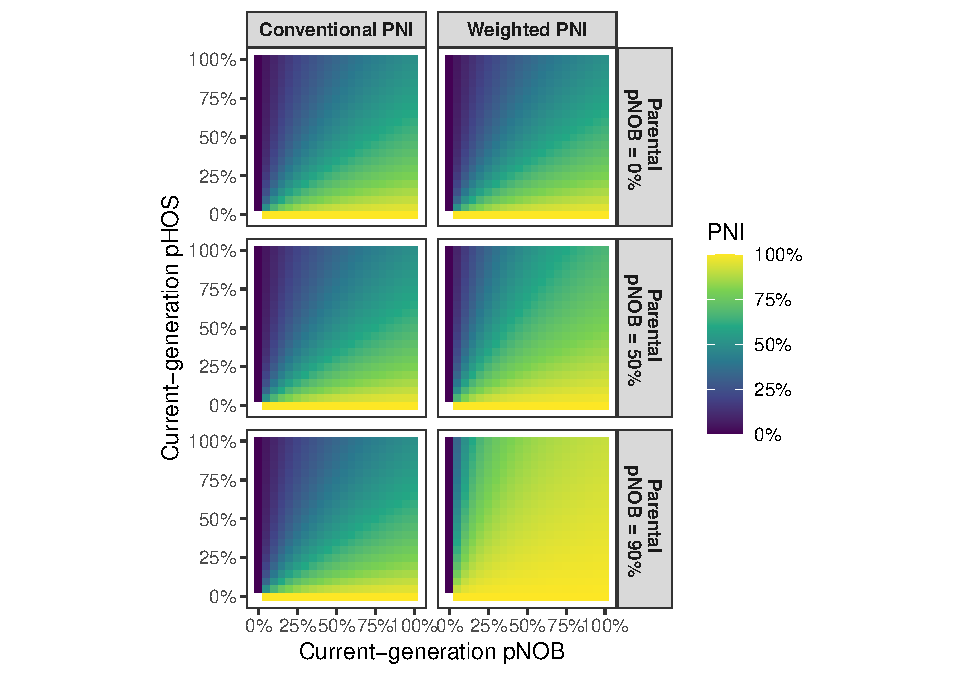
\includegraphics[width=1\linewidth]{NEOR_proposed_weir_mgt_files/figure-latex/compare-pni-1} 

}

\caption{Estimated PNI values using the current calculation method and a weighted method using parental pNOB as the weight.}\label{fig:compare-pni}
\end{figure}

\begin{figure}[H]

{\centering 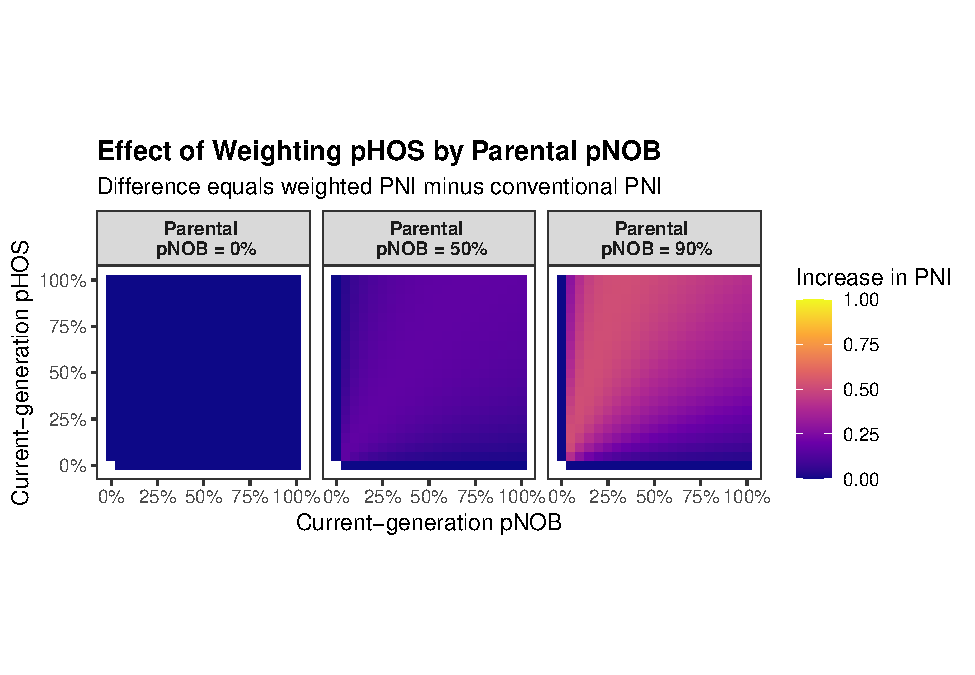
\includegraphics[width=1\linewidth]{NEOR_proposed_weir_mgt_files/figure-latex/pni-differnce-1} 

}

\caption{Difference in PNI values using the current calculation method and a weighted method using parental pNOB as the weight.}\label{fig:pni-differnce}
\end{figure}

% References (only if bibliography present)
\section*{References}
\printbibliography[heading=none]


\end{document}
